\documentclass[10pt]{article}
%\usepackage[french]{babel}
\usepackage{fontspec}
\usepackage{polyglossia}
\setdefaultlanguage{french}
\usepackage[a4paper,margin=2cm]{geometry}
\usepackage{url,hyperref}
%\usepackage{siunitx}
%\usepackage{schemabloc}
%\usepackage{listings}
%\usepackage{auto-pst-pdf}
%\usepackage{pst-circ}
%\usepackage{soul}
%\usepackage{verbatim}
\usepackage{lmodern}
%\usepackage{tikz}
%\usepackage[european,cuteinductors,siunitx]{circuitikz}
\usepackage{xunicode,xltxtra}
\usepackage{graphicx}
\usepackage{amsmath}
\usepackage{minted}
%\usepackage{multicol}
\title{
\includegraphics{inp-enseeiht} \\ ~ \\ ~ \\ ~ \\ ~ \\ Exercices de Matlab \\ ~ \\ Quatrième séance \\ ~ \\ Exercices de SIMULINK}
\author{Guilhem Saurel}
\date{\today}
\renewcommand{\thesubsection}{\thesection .\Alph{subsection}}
\begin{document}

 \begin{titlepage}
  \maketitle
  \tableofcontents
 \end{titlepage}

 \section{Visualisation d’un signal bruité}
  \subsection{}
   \begin{center}
    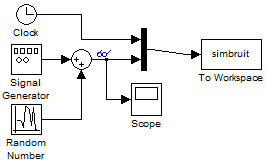
\includegraphics{1a}
   \end{center}
  \subsection{}
   \begin{center}
    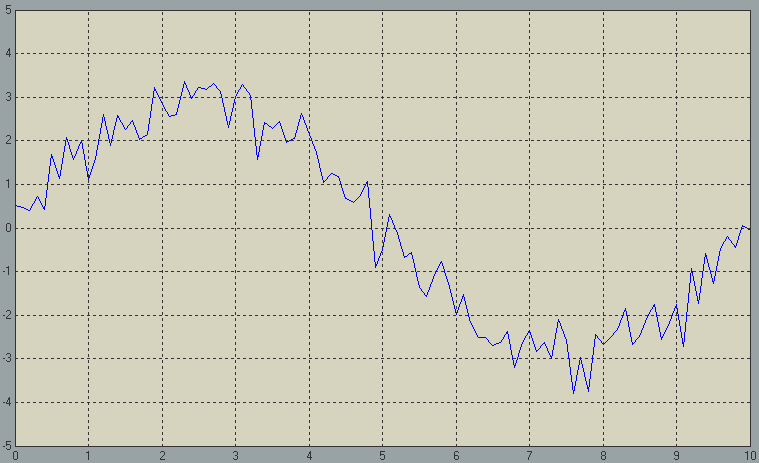
\includegraphics[width=8cm]{1b}
   \end{center}
  \subsection{}
   \inputminted{matlab}{1c.txt}
  \subsection{}
   On peut visualiser le signal sinusoïdal à l’aide d’un plot %\mint|plot(simbruit(:,2))| :
   \begin{center}
    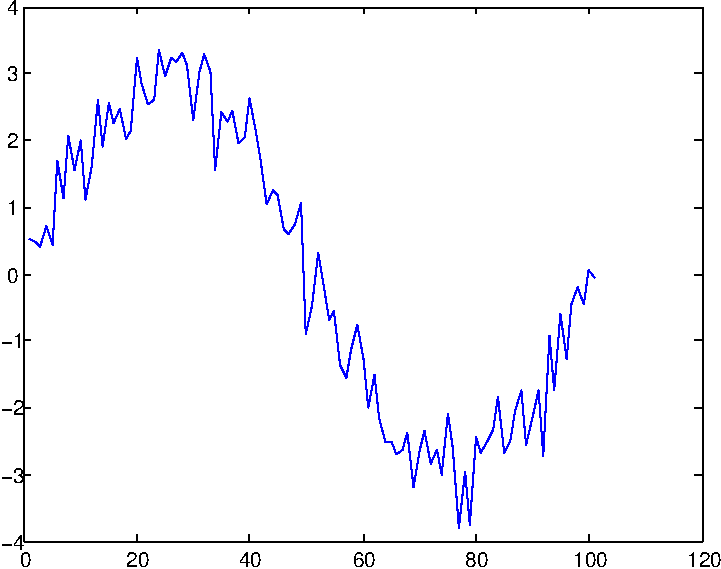
\includegraphics{1d}
   \end{center}
   Ou via l’oscilloscope :
   \begin{center}
    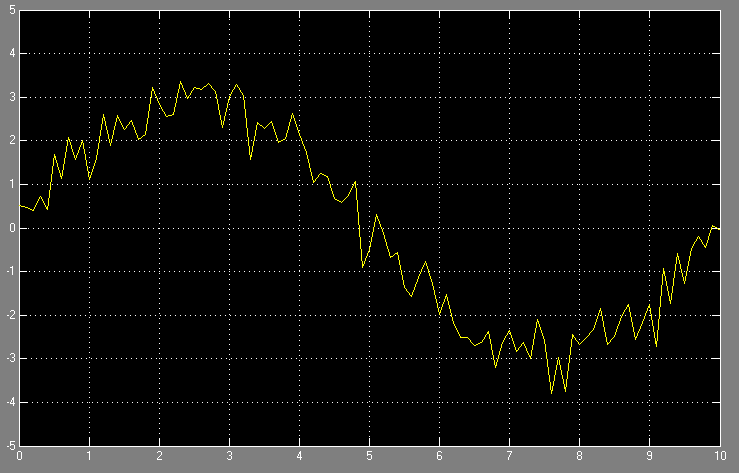
\includegraphics[width=16cm]{1d_scope}
   \end{center}
 \section{Simulation à partir de la fonction de transfert}
  \begin{center}
   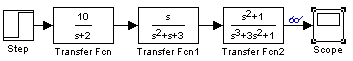
\includegraphics{2_sb}
   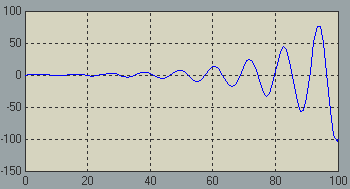
\includegraphics{2_simu}
  \end{center}
 \section{Analyse temporelle et fréquentielle d’un système de deuxième ordre}
  \subsection{}
   $
    \left. \begin{array}{c c c}
     \omega_0 &=& 1 \\
     \xi &=& 0.1
    \end{array} 
    \right\} 
    \Rightarrow
    \cfrac{1}{1+\cfrac{2\xi}{\omega_0} p+\cfrac{p^2}{\omega_0^2}} = \cfrac{1}{p^2+0,2p+1}
   $
   \begin{center}
    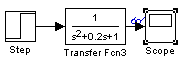
\includegraphics{3a_1}
    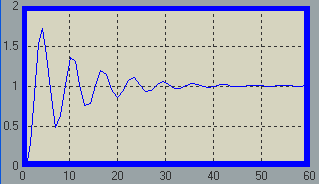
\includegraphics{3a_1-s}
   \end{center}
   $
    \left. \begin{array}{c c c}
     \omega_0 &=& 2 \\
     \xi &=& 0.707
    \end{array} 
    \right\} 
    \Rightarrow
    \cfrac{1}{1+\cfrac{2\xi}{\omega_0} p+\cfrac{p^2}{\omega_0^2}} = \cfrac{1}{0.25p^2+0,707p+1}
   $
   \begin{center}
    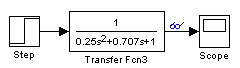
\includegraphics{3a_2}
    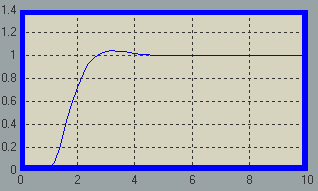
\includegraphics{3a_2-s}
   \end{center}
   $
    \left. \begin{array}{c c c}
     \omega_0 &=& 3 \\
     \xi &=& 2
    \end{array} 
    \right\} 
    \Rightarrow
    \cfrac{1}{1+\cfrac{2\xi}{\omega_0} p+\cfrac{p^2}{\omega_0^2}} = \cfrac{1}{p^2+12p+9}
   $
   \begin{center}
    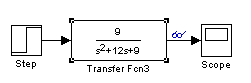
\includegraphics{3a_3}
    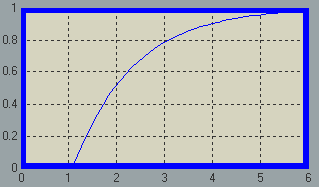
\includegraphics{3a_3-s}
   \end{center}

 \section{Générateur de signaux périodiques}
  \subsection{}
   On incrémente la constante n dans le bloc suivant jusqu’à obtenir un carré acceptable :
   \begin{center}
    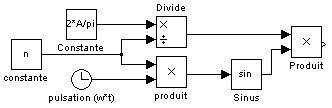
\includegraphics{4a}
   \end{center}
   Pour 5 blocs tels que celui-ci (et donc les harmoniques 1 3 5 7 et 9), on obtient :
   \begin{center}
    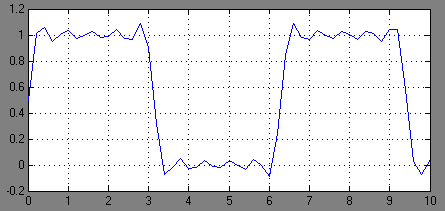
\includegraphics{4a-s}
   \end{center}
  \subsection{}
   De la même manière, on incrémente la constante n dans le bloc suivant jusqu’à obtenir un triangle acceptable :
   \begin{center}
    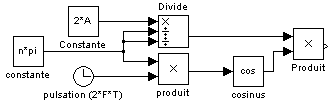
\includegraphics{4b}
   \end{center}
   Cette fois-ci, pour le triangle, deux harmoniques suffisent
   \begin{center}
    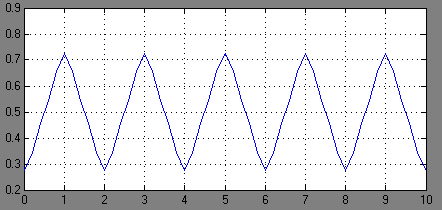
\includegraphics{4b-s}
   \end{center}
   Naturellement, le rendu sous MATLAB est le même :
   \begin{center}
    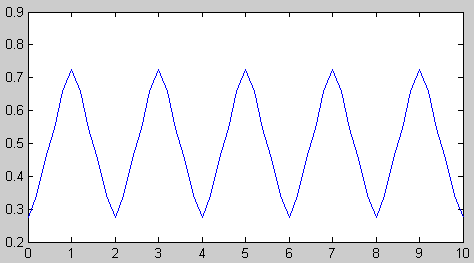
\includegraphics{4b-p}
   \end{center}

 \section{Sinus cardinal}
  \subsection{}
   \begin{center}
    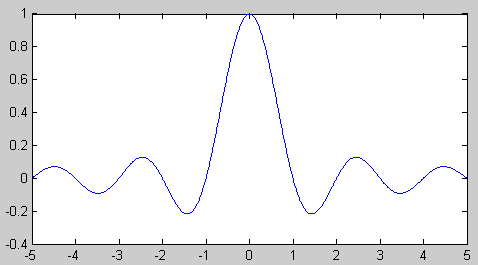
\includegraphics{5a}
   \end{center}
  \subsection{}
   \begin{center}
    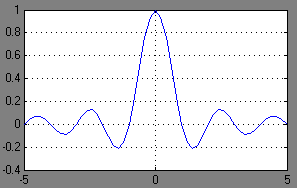
\includegraphics{5b}
   \end{center}

 \section{Fonctions logiques}
  \subsection{}
   \begin{tabular}{|c|c|c|}
    \hline
    B/A&0&1\\
    \hline
    0&1&1\\
    \hline
    1&1&0\\
    \hline
   \end{tabular}
   On peut donc simplifier $X=A\oplus B+\overline{A+B}=\bar A + \bar B$
  \subsection{}
   \begin{center}
    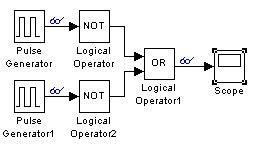
\includegraphics{6b}
   \end{center}
  \subsection{}
   \begin{center}
    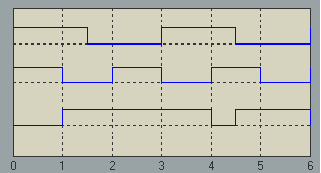
\includegraphics{6c}
   \end{center}

\end{document}
